\documentclass[11pt]{extarticle}
\usepackage{fullpage}
\usepackage[ampersand]{easylist}
\ListProperties(Hide=10, Style*=$\bullet\;\,$, Style2*=$\;\,${\tiny$\blacksquare$}$\;\,$,Space*=0.5mm,Space2*=0mm)

\usepackage{amsmath}
\usepackage{amssymb}
\usepackage{amsthm}
\newtheorem{thn}{Theorem}[]
\usepackage{mathtools}
\usepackage{bibref}

\usepackage[T1]{fontenc}
%\usepackage{newtxtext}
\usepackage[vvarbb]{newtxmath}

\usepackage{tikz}
\usetikzlibrary{calc}
\usetikzlibrary{shapes}
\usepackage{pgfplots}
\pgfplotsset{trig format plots=rad}

\usepackage[p,osf]{scholax}
\usepackage{multicol}
\setlength{\columnsep}{0.5cm}
%\setlength\columnseprule{.1pt}

\newcommand{\R}{\mathbb{R}}
\newcommand{\C}{\mathbb{C}}
\newcommand{\Na}{\mathbb{N}}
\newcommand{\ra}{\rightarrow}
\newcommand{\w}[1]{\text{#1}}
\newcommand{\sm}[2]{\displaystyle\sum_{#1}^{#2}}
\author{Yashas.N}
\title{Special examples}
\date{}
\begin{document}
	\maketitle
	\boldmath
	\section{Sequences and Series}
	\begin{easylist}[enumerate]
	& Riemann-Zeta function $\zeta:\C \ra \C+\infty$ defined by
	\[\zeta(s)=\sm{n=1}{\infty}\frac{1}{n^s}\]
	&& if $1< Re(s)<\infty$ then the series converges uniformly and absolutely 
	&& clearly $\zeta$ is analytic for $Re(s)>1$
	&& \textbf{Euler's Product formula}:
	\[\zeta(z)=\prod \left(1-\frac{1}{p^s}\right)^{-1}\]
	where the product ranges over all primes $p$ which implies $\zeta(s)\neq 0$ if $Re(s)>1$. More generally we have
	\[\zeta(s)(1-2^{-s})(1-3^{-s})\dots (1-p_N^{-s})=\sum m^s=1+p_{N+1}^{-s}\dots\]
	where the R.H.S ranges for all $+ve$ integers that contain none of prime factors $2,3,\dots,p_N$
	&& now if $1<s<\infty$ (i.e. $s$ is real $>1$) then 
	\[\zeta(s)=s\int_{1}^{\infty}\frac{[x]}{x^{s+1}}dx\]
	where $[x]$ is greatest integer $\leq x$
	&& more generally if $Re(s)>1$ then 
	\[\zeta(s)=\frac{1}{\Gamma(s)}\int_{0}^{\infty}\frac{x^{s}-1}{e^x-1}dx\]
	where $\Gamma(z)$ is defined by product representation for complex numbers.
	
	& $\sm{n=1}{\infty}\frac{(-1)^{n+1}}{n}$ 
	&& is convergent to $\ln(2)$ 
	&& does not converge absolutely.
	\end{easylist}

	\section{Functions in $\R$}
	\begin{easylist}[enumerate]
	& Dirichlet Function $\delta(x)$
	\end{easylist}
	\[ \delta(x)=
	\begin{cases}
	1 & \quad \w{ if } x \w{ is rational}\\
	0 & \quad\w{ if } x \w{ is irrational}\\
	\end{cases} \]
	\begin{easylist}
	&& $\delta$ is not Riemann Integrable in any interval $[a,b]$
	&& $\delta$ is Lebesgue Intergrable in $\R$ and has $0$ integral value with usual lebesgue measure as the set for which $\delta$ is not zero is countable.
	& $f:\R \ra \R$ such that for every rational $r=m/n$ where $n>0$ and $m,n\in \mathbb{Z}$ with out any common divisors then $f(r)=f(m/n)=1/n$ , $x=0$ take $n=1$ i.e. $f(0)=1$ and $f(x)=0$ if $x$ is irrational i.e.
	\end{easylist}
	\[ f(x)=
	\begin{cases}
		0 & \quad \w{if } x \w{ is irrational}\\
		\frac{1}{n} & \quad\w{ if } x=\frac{m}{n}\\
	\end{cases} \]
	\begin{easylist}
		&& $f(x)$ is continuous at every irrational number
		&& $f(x)$ is discontinuous at rational with simple discontinuities
		%	\newpage
		& $\sin(x)$
	\end{easylist}
	\begin{multicols}{2}
	\begin{easylist}
		&& can be defined without geometric interpretation as \\
		$\sin x = (e^{ix}-e^{-ix})/2$ for real $x$ 
		&& $\sin$ is continuous one-one function in domain $[-\pi,\pi]$ onto $[-1,1]$  hence inverse $\sin^{-1}$ is defined in this area.
		&& we see that $\frac{2}{\pi}x\leq \sin x \leq x$ holds  $\forall x\in[0,\pi/2]$
		
		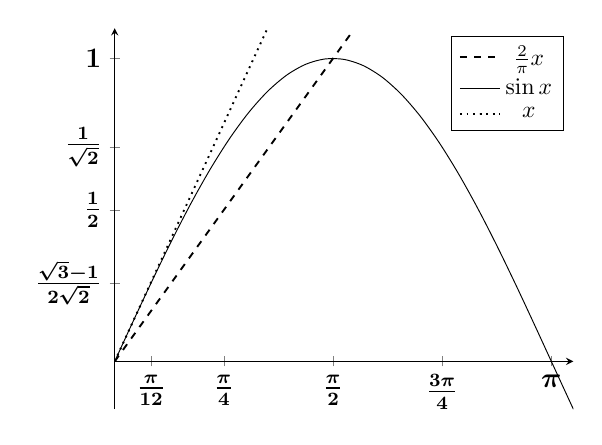
\begin{tikzpicture}[scale=.85]
			\begin{axis} [axis lines=middle,
				tick label style = {font=\large\boldmath},
				domain=0:3.3,
				xtick ={0,pi/12,pi/4,pi/2,3*pi/4,pi},
				xticklabels={0,$\frac{\pi}{12}$,$\frac{\pi}{4}$,$\frac{\pi}{2}$,
					$\frac{3\pi}{4}$,$\pi$},
				ytick ={0,0.2588,0.5,1/1.4142,1},
				yticklabels={0,$\frac{\sqrt{3}-1}{2\sqrt{2}}$,$\frac{1}{2}$,
					$\frac{1}{\sqrt{2}}$,$1$},
			legend entries ={$\frac{2}{\pi}x$,$\sin x$,$x$}]
		\addplot [thick,dashed,domain=0:1.7]{2*x/pi};
		\addplot[smooth,domain=0:3.3] {sin(x)};
		\addplot [thick,dotted,domain=0:1.1] {x};
		
			\end{axis}
			\end{tikzpicture}
	\end{easylist}
		\end{multicols}
\begin{easylist}
	& Distance to a closed set function
	&& if $ A $ is any closed set in $ \R $ define $ D_A(x)=\inf(d(x,a)) $ for $ a\in A $ and a metric $ d $ on $ \R $ (usually the Euclidean metric). 
	&& for $ x,y\in \R $ say $ \inf(d(a,x)) $ for $ a\in A $ occurs at $ p\in A $ and  $ \inf(d(a,y))$ for $ a\in A $ occurs at $ q\in A $ i.e. $ |D_A(x)-D_A(y)|=|d(p,x)-d(q,y)| $ (this is possible since $ A $ is closed in $ \R $ ) now as $ d(q,y)\leq d(p,y) $ we have  $|D_A(x)-D_A(y)|\leq |d(p,x)-d(p,y)|\leq |d(x,y)| $ as $ d(p,x)\leq d(p,y)+d(x,y) $ so we get if $ d(x,y)<\epsilon $ then $|D_A(x)-D_A(y)|<\epsilon $ thus $ D_A $ is uniformly continuous.
	&& Thus there exist a uniformly continuous function of $ \R $ that has zeroes exactly equal to a given closed set in $ \R $ (namely $ D_A$ for a given closed set $ A\subset \R $).
\end{easylist}


	
\end{document}